% Toolbar icon: ptStructural — the Structural Mechanics problemtype logo:
% a cantilever beam clamped at a hatched wall with a tip load arrow.
% NOTE: the committed svg-ui/ptStructural.svg was hand-authored to the same
% drawing (no LaTeX toolchain available); regenerating via `make ui` replaces
% it with the pdftocairo rendering of this source — same glyph either way.
\documentclass[tikz,border=2mm]{standalone}
\usetikzlibrary{arrows.meta,calc,shapes.geometric}
\begin{document}
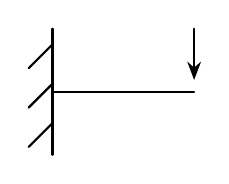
\begin{tikzpicture}[line width=1.3pt, line cap=round, line join=round, >=Stealth, x=1mm,y=1mm]
  % clamped wall + hatching
  \draw[thick] (-9,-8) -- (-9,8);
  \foreach \y in {-7,-2,3} {
    \draw[thick] (-12,\y) -- (-9,\y+3);
  }
  % beam
  \draw[thick] (-9,0) -- (9,0);
  % tip load
  \draw[thick,->] (9,8) -- (9,1.5);
\end{tikzpicture}
\end{document}
